% !TEX root = Master.tex

Simple maximum likelihood estimation based on the log-sales of the margins allow us to estimate the ex-Gaussian distribution parameters. \autoref{fig:kcc_2_density} describes how the histogram of the data match to the theoretical density of an ex-Gaussian distribution. The estimated parameter values are $\hat{\mu} = 7.85$, $\hat{\sigma} = 0.26$ and $\hat{\nu} = 0.33$.
\\
%represented in \autoref{tab:estimated_parameters_kcc_2_no_covariates}.





%\begin{table}[H]
%\setlength\arrayrulewidth{1pt}  
%\centering
%\begin{adjustbox}{max width=\textwidth}\
%\begin{tabular}{|c|c|c|}
%\hline
%\rowcolor{lightgray} 
%$\hat{\mu}$ & $\hat{\sigma}$ & $\hat{\nu}$ \\ \hline
%7.85        & 0.26           & 0.33        \\ \hline
%\end{tabular}
%\end{adjustbox}
%\caption{Estimated parameters for log-sales of KCC 2 fitted to ex-Gaussian distribution with no covariate effects}
%\label{tab:estimated_parameters_kcc_2_no_covariates}
%\end{table}





 \begin{figure}[H]
\centering
\begin{subfigure}{.45\textwidth}
  \centering
  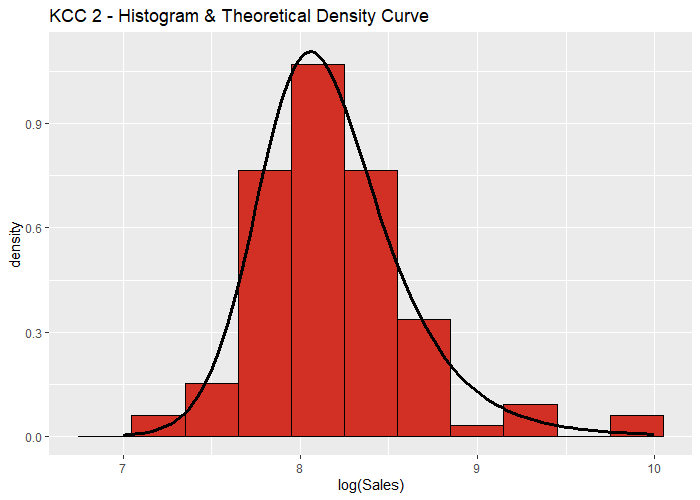
\includegraphics[width=\linewidth]{figures/kcc_2_density.png}
  \caption{Histogram \& theoretical density}
  \label{fig:kcc_2_density}
\end{subfigure}
\begin{subfigure}{.45\textwidth}
  \centering
  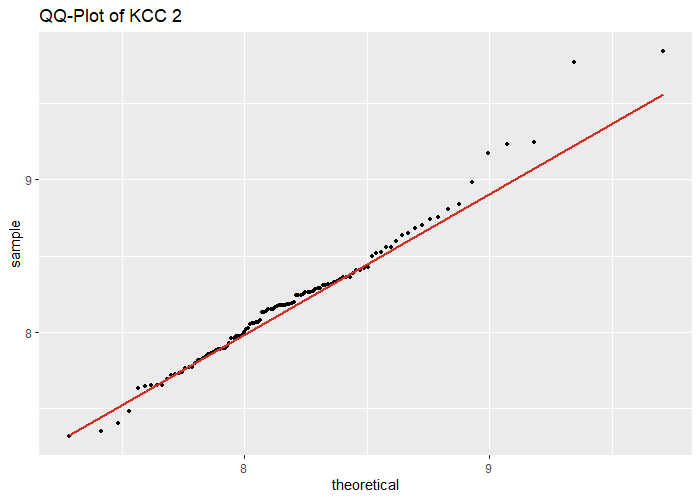
\includegraphics[width=\linewidth]{figures/kcc_2_qqplot.png}
  \caption{QQ-plot}
  \label{fig:kcc_2_qqplot}
\end{subfigure}
\caption{ex-Gaussian distribution fitted to log-sales of \ac{KCC} 2}
\label{fig:kcc_2_margin}
\end{figure} 




\begin{figure}[H]
\centering
  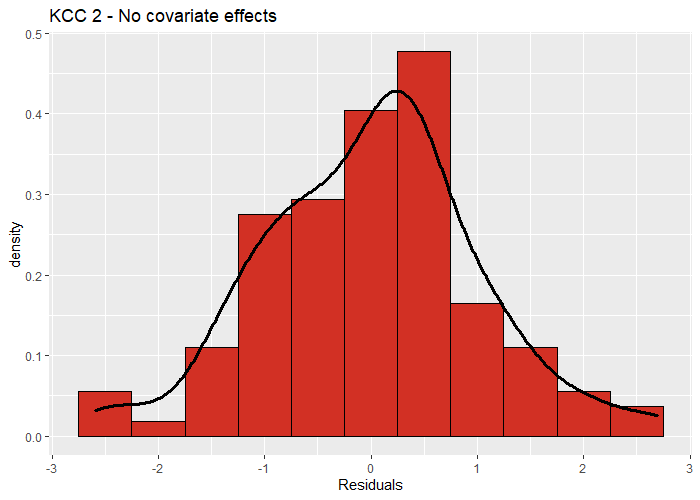
\includegraphics[width=0.45\linewidth]{figures/res_kcc_2_no_covariates.png}
  \caption{Residuals of KCC 2 log-sales fitted to an ex-Gaussian distribution with no covariate effects together with their density curve}
  \label{fig:res_kcc_2_no_covariates}
\end{figure}

As can be seen in \autoref{fig:res_kcc_2_no_covariates}, the residuals of the fitted distribution are not too far from a normal distribution. 
In fact, a Shapiro-Wilk normality test (see Section \ref{ssec:shapiro_wilk}) fails to reject the null hypothesis, returning a p-value of 0.6645.
There still exist skewness in the distribution of the residuals and correction is attempted in the following. 
\\

The findings so far indicate that the overall fit for this cluster is quite satisfiable and also supports interpretability of the estimated parameters. \\
To make the estimation more precise and to get a better understanding of what is driving sales, flexible estimation of the distribution parameters is required and thus covariate effects shall be included. \\
%The temporal effects in particular are of special interest. 

After multiple equation setups for the marginal distribution of \ac{KCC} 2, the chosen \ac{GAMLSS} model specification (see Section \ref{ssec:gamlss}) is as follows:
\begin{equation}
\begin{aligned}
\mu &= \beta_{\mu} + f_{\mu , 1}(\textit{time}) + f_{\mu ,2}(\textit{total\_markdown\_pct}) + \\
 & \quad \textit{promo\_type*total\_markdown\_pct} \\ \noalign{\vskip5pt}
log(\sigma) &= \beta_{\sigma} + f_{\sigma}(\textit{time}) \\ \noalign{\vskip5pt}
log(\nu) &=  \beta_{\nu}, 
\end{aligned}
\label{eq:gamlss_kcc_2}
\end{equation} 

where \textit{promo\_type} is a factor variable with levels \textit{"No Promotion"} (reference category), \textit{"Black Friday"} and \textit{"Friends \& Family"}. The smooth functions $f_{\mu ,1}$, $f_{\mu ,2}$ and $f_{\sigma}$ are build upon P-splines with 40 knots each. For the scale and shape parameters ($\sigma$ and $\nu$ respectively) the logarithmic link function is used to ensure that they are mapped to the real positive line as the ex-Gaussian distribution family can only capture positive skewness ($\nu$). For $\sigma$ we just use time as the only regressor and we set the skewness $\nu$ as a constant.\\
 The estimated location and scale parameters over time are depicted in \autoref{fig:gamlss_kcc_2_estimated_parameters} and in \autoref{tab:nu_ci_kcc_2} the estimated skewness parameter value with its 95\% confidence interval is shown. The fitted values approximate the actual values quite adequately given the present limitations. The sale peaks are also well captured, especially for Black Friday. The scale parameter has an increasing trend up until roughly mid-January (60th observation) and then decreases again. However, the overall range of deviation is kept to a minimum, ranging from 0.05 to 0.20. The estimated skewness parameter is closer to zero than in the maximum likelihood approach without any covariate effects.
\\


\begin{figure}[H]
\centering
  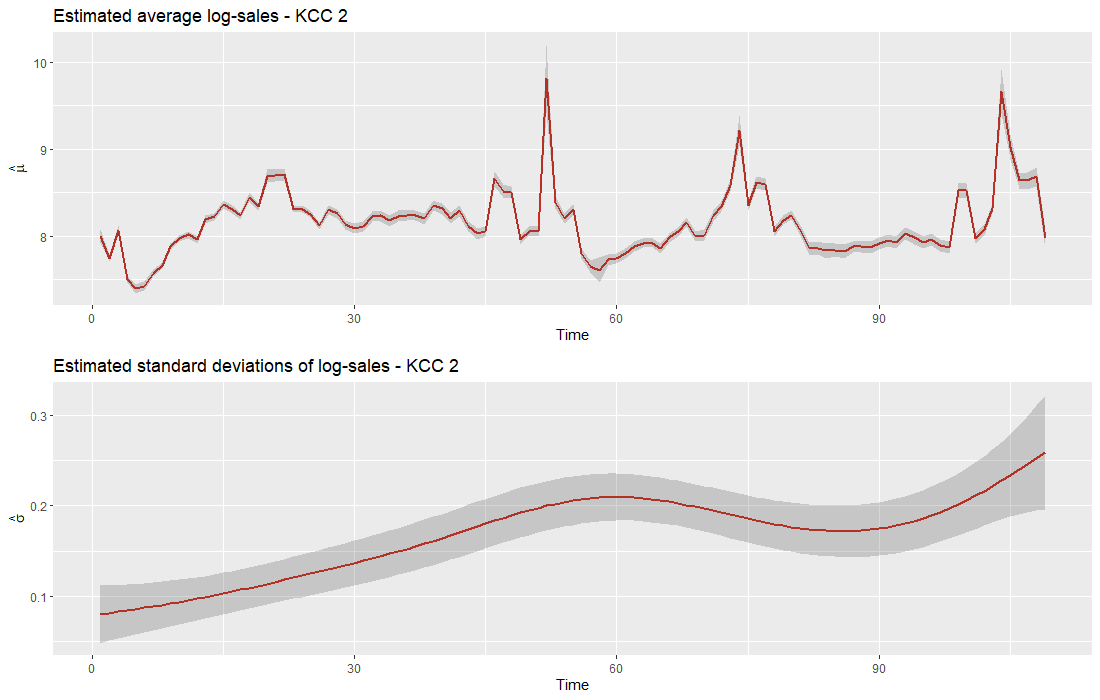
\includegraphics[width=0.95\linewidth]{figures/gamlss_kcc_2_estimated_parameters.png}
  \caption{Estimated location parameter $\hat{\mu}$ compared to the observed values and scale parameter $\hat{\sigma}$ with confidence bands of GAMLSS fit - KCC 2}
  \label{fig:gamlss_kcc_2_estimated_parameters}
\end{figure}





\begin{table}[H]
\setlength\arrayrulewidth{1pt}  
\centering
\begin{adjustbox}{max width=\textwidth}\
\begin{tabular}{c|c|c}
\hline
\rowcolor{white} 
\textbf{Lower} & $\hat{\nu}$ & \textbf{Upper} \\ \hline\hline
0.067        & 0.058           & 0.076        \\ \hline
\end{tabular}
\end{adjustbox}
\caption{Estimated skewness parameter $\hat{\nu}$ of GAMLSS fit with 95\% confidence interval bounds - KCC 2}
\label{tab:nu_ci_kcc_2}
\end{table}



%The absence of the Black Friday and Friends \& Family components in Model \ref{eq:gamlss_kcc_2} is due to the fact that the effects of activated promotions to the expected sales are negative, which is contradictory to the analysis made earlier in Chapter \ref{ssec:grouped_patterns}. The output after excluding those indicator variables seem to be more stable and is also more intuitive.\footnote{This might be traced back to the fact that promos obviously yield higher markdowns and thus we reach redundancy of variables in the model.} 


The estimated coefficients of the \ac{GAMLSS} fit on the log-sales of \ac{KCC} 2 with standard errors and significance codes are displayed for $\hat{\mu}$ in \autoref{tab:gamlss_coeff_kcc_2}. A detailed summary of the resulting output can be found in the Appendix (R output \ref{output:gamlss_fit_kcc_2_try20}).
\\


\begin{table}[H]
\centering
\begin{tabular}{l|c|c|c|l}
  \hline
  \rowcolor{white}
 \textbf{$\hat{\mu}$ Coefficients} & \textbf{Estimate} & \textbf{Std. Error} & \textbf{t value} & \textbf{p-value} \\ 
  \hline\hline
\textit{$\beta_{\mu}$ (Intercept)} & 5.54 & 0.07 & 75.90 & 0.00 *** \\ 
  \textit{$f_{\mu, 1}$(time)} & 0.00 & 0.00 & 3.83 & 0.00 *** \\ 
  \textit{$f_{\mu ,2}$(total\_markdown\_pct)} & 6.79 & 0.18 & 36.77 & 0.00 *** \\ 
  \textit{promo\_typeBlack Friday} & 1.33 & 0.19 & 7.02 & 0.00 *** \\ 
  \textit{promo\_typeFriends \& Family} & 2.31 & 0.41 & 5.56 & 0.00 *** \\ 
  \textit{promo\_typeBlack Friday:total\_markdown\_pct} & -3.87 & 0.37 & -10.54 & 0.00 *** \\ 
  \textit{promo\_typeFriends \& Family:total\_markdown\_pct} & -6.10 & 0.75 & -8.13 & 0.00 *** \\ \hline
\end{tabular}
\caption{Estimated $\hat{\mu}$ coefficients of \ac{GAMLSS} fit on log-sales of \ac{KCC} 2}
\label{tab:gamlss_coeff_kcc_2}
\end{table}

%Below we can observe the summary output from the R console (R output \ref{output:gamlss_fit_kcc_2_try20} as well as the visual covariate effects on the expected value (\autoref{fig:gamlss_effects_kcc_2}).




%\VerbatimInput[label = "GAMLSS Fit on KCC 2" ]{gamlss_fit_kcc_2_try20.txt}






From the visual representation of the covariate effects in (\autoref{fig:gamlss_effects_kcc_2}, we can see that the temporal effect on log-sales varies within a certain range.
% until about August of 2017 (just below the 40th time observation) the log-sales are increasing and then from November on (roughly 50th observation) the log-sales remain at a constant level with somewhat higher values end of May (just below 80th observation). The overall course of the temporal effect on the response resembles a flat wavy line around zero, which is quite aligned with the coefficient in the R-output. 
Higher total markdown percentages enhance higher response values, which can also be observed when looking at \autoref{tab:gamlss_coeff_kcc_2}. The estimated coefficient for the markdown obtains a value of 6.79 (without considering promotions). The log-sales increase by 1.33 and 2.31 units on average when Black Friday and Friends \& Family respectively is activated, assuming no total markdown percentages exist. That is of course counterintuitive, as promotion go hand in hand with markdowns. The summary in \autoref{tab:gamlss_coeff_kcc_2} reveals such kind of peculiar effects when we look at the interaction coefficients of promotions and total markdown percentage. When any promo type is activated, the total markdown percentage has a negative effect on the log-sales. Interpretation of the results shall be expressed with caution. Season type (SS \& FW) was not included in the model as it had no significant effect and distorts the output and the effect plots. All curves of smooth effects are centered around zero due to identifiability constraints (see Section \ref{ssec:gam}).
%The seasonal effect of Spring-Summer is slightly lower than the effect of Fall-Winter. 
%The estimated standard error $\hat{\sigma}$ is generally increasing over time in this data spectrum (\autoref{fig:sigma_effect_kcc_2}). 
\\



\begin{figure}[H]
\centering
  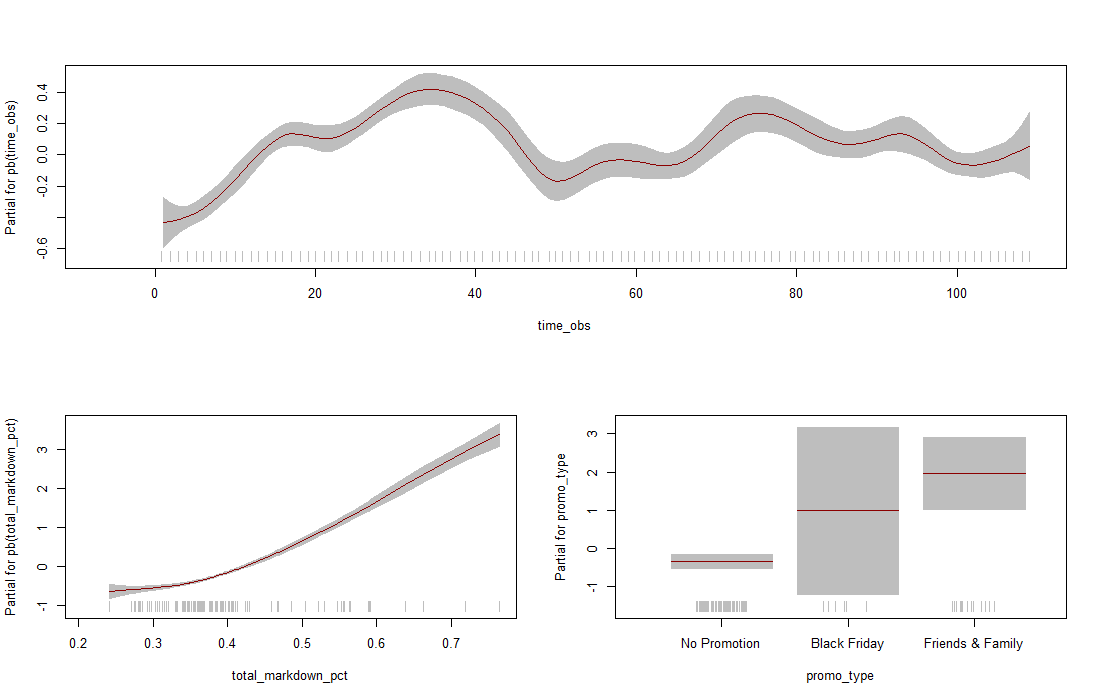
\includegraphics[width=0.95\linewidth]{figures/gamlss_effects_kcc_2.png}
  \caption{Covariate effects on the expected response variable (log-sales) of GAMLSS fit - KCC 2}
  \label{fig:gamlss_effects_kcc_2}
\end{figure}




\begin{figure}[H]
\centering
  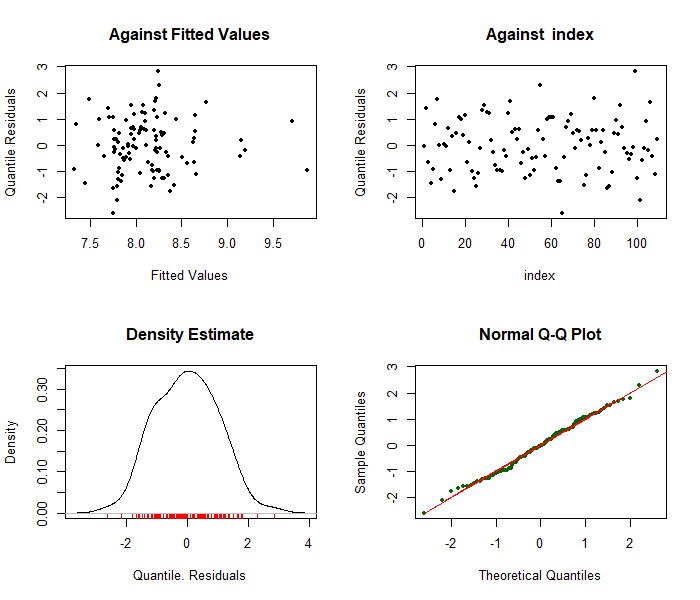
\includegraphics[width=0.95\linewidth]{figures/gamlss_residuals_kcc_2.png}
  \caption{Residuals of GAMLSS fit - KCC 2}
  \label{fig:gamlss_residuals_kcc_2}
\end{figure}



Fitting the data to a \ac{GAMLSS} model like this can be considered favourable. The emerged residuals are closer to a standard normal distribution than the maximum likelihood estimation without any covariate effects. Diagnostic plots of quantile residuals in \autoref{fig:gamlss_residuals_kcc_2} confirm this. \autoref{tab:gamlss_residuals_kcc_2} returns a detailed summary of the estimated location, scale and shape parameters of the residuals' distribution. The mean, variance, skewness and kurtosis are close enough to zero, one, zero and three respectively, which are sufficient conditions to assume normality for practical purposes. A Shapiro-Wilk test for the newly emerged residuals returns a p-value of 0.92, which is also in plain favour of a normal distribution.
\\




\begin{table}[H]
\centering
\begin{tabular}{c}
\hline
\rowcolor{white} 
\textbf{Summary of the Quantile Residuals} \\ \hline\hline
 $\begin{array}[t]{ r @{{}={}} l }
\text{mean} & -0.01811135                         \\ 
\text{variance} & 1.042057                        \\ 
\text{coef. of skewness} & 0.08348086             \\ 
\text{coef. of kurtosis} & 2.645021               \\ \hline
\end{array}$
\end{tabular}
\caption{Residuals of GAMLSS Fit on KCC 2}
\label{tab:gamlss_residuals_kcc_2}
\end{table}




%\inputRoutput[caption={Residuals of GAMLSS Fit on KCC 2},numbers=left,numberstyle=\tiny, label=output:gamlss_residuals_kcc_2]{gamlss_residuals_kcc_2.txt}